\documentclass[9pt]{IEEEtran}

\usepackage{graphicx}
\usepackage{subcaption}
\usepackage{pdfpages}

\usepackage{array}
\newcolumntype{x}[1]{>{\centering\arraybackslash\hspace{0pt}}p{#1}}

\title{AI-Guided Game Design for the Game ``Space Battle''}
\author{Matthew Bedder, Athanasios Kokkinakis, Andrei Iacob, Mihail Morosan}
	
\usepackage[backend=bibtex, style=ieee]{biblatex}

\usepackage{amssymb}

\addbibresource{GD2_bib.bib}

\begin{document}



\maketitle
%%%%%%%%%%%%%%%%%%%%%%%%%%%%%%%%%%%%%%%%%%%%%%%%%%%%%%%%%%%%%%%%%%%%%%%%%%%%%%%

\begin{abstract}

In this study we propose two variations on a game designed to improve player experience, and we use both AI agents and testing with human players to try to demonstrate that the game variants improve the players' experience. For the AI agents, a number of metrics are recorded from AI versus AI gameplay, and some simple analytics used to see if the intended impact is achieved. We then use human players to try to confirm these results, and to try to demonstrate the usefulness of using analytics over AI gameplay to measuring the impact to changes on video games. No relevant correlation was found between results inferred from AI testing and results from human testing.

\end{abstract}

\section{Introduction}
Improving the player experience has been the main goal of game designers since the beginning of the computer games industry. A plethora of techniques have been used into try to achieve this, of which some approaches  have proven to be very effective, and others less so.

In this study we propose two variations on a game designed to improve player experience, and use both AI agents and testing with human players to try to demonstrate that the game variants improve the player experience. For the AI agents, a number of metrics are recorded from AI versus AI gameplay, and some simple analytics used to see if the intended impact is achieved. We then use human players to try to confirm these results, and to try to demonstrate the usefulness of using analytics over AI gameplay to measuring the impact to changes on video games.

In the first instance, intelligent agents were used to play the game and a number of game metrics and analytics were collected in order to quantify their experience. In the second part of the project, human players were asked to participate in an experiment, playing three different versions of the game, one being the classical battle, and the other two versions containing incremental modifications and increased complexity. The human players were asked to fill in a questionnaire while playing through each version of the game, in order to understand their gaming experience and their responses to the changes in the mechanics of the game brought by the modified versions.

%%%%%%%%%%%%%%%%%%%%%%%%%%%%%%%%%%%%%%%%%%%%%%%%%%%%%%%%%%%%%%%%%%%%%%%%%%%%%%%
\section{Existing work}
\subsection{Player experiences of games}

Recently there has been much work into using automated methods for optimising game designs. Work by Isaksen et al. (Exploring Game Space using Survival Analysis)(Discovering unique game variants) has looked into using survival analysis to optimising parameters defining gravity and jump force in the game “Flappy Bird”. Using their technique, a simple, partially stochastic AI agent is made to play the game for a parameter set a number of times, with the distribution of the scores achieved by the agent being recorded. These score distributions can then be recorded for a number of different sets of parameter values, and these distributions used to select sets of parameters that provide gameplay fitting some criteria (with potential criteria including the difficulty of the game, and the “uniqueness” of the gameplay provided by the parameter set. This reduces the need for the game designer to explore the space of the parameter set manually, and suggests that the results of automated playtesting correlate with human players' experience with the game.

Aside from using automated playtesting to test parameter values, it can also be used to assess different sets of game mechanics. Work by Nelson et al. looked into using AI players to evaluate mechanics of procedurally generated games (Rules and mechanics). In this approach it was found that the automatic generation of criteria about the playability of the game were effective when combined with a genetic programming approach for automatically generating game rule sets. In many of these approaches, the criteria used for assessing the quality of games have been relatively complex in order to try to capture the subtleties of player experience, including metrics on whether game states that appear advantageous often result in the player winning (Rules and Mechanics) or whether the player's ability to significantly impact the score they will achieve (Multi-Faceted Evolution Of Simple Arcade Games).

\subsection{AI-based game design}

The reasons behind why people enjoy particular videogames but are uninterested in others has remained elusive, despite numerous attempts to quantify them (Yannakakis, 2005 Procci, 2012 Chell, 2008). A generally agreed accepted principle is that of similarly skilled opponents, whether they are human or A.I. generated, who are challenging enough for the player to keep him focused in the game while being realistically beatable so that the player does not experience frustration or even anxiety (Ibanez \& Mata, 2011).

Human performance in relatively simple videogames that rely on reaction times has been the Learning Strategies Program, originally funded by the Defense Advanced Research Projects Agency (Donchin et al., 1989). This program gave birth to the Space Fortress game, a game that  largely resembles Asteroids (Boot, 2015). Subsequent examinations of this game showed that Attention, Working Memory and even Fluid Intelligence all highly correlated with game performance (Rabbit et al., 1989). All the aforementioned variables are highly mediated by a multitude of individual differences such as gender, nationality, age, socioeconomic status, handedness, working memory and even language (Lyle, Roediger \& McCabe, 2008; Cazzato et al., 2010; Stigler, 1986; Templer \& Stephens, 2014; Greiner, Schoenfield \& Liepert, 2014).Thus the selection and development of the appropriate A.I. agents, fitted to players’ individual differences, is imperative for maximising user experience. 

%%%%%%%%%%%%%%%%%%%%%%%%%%%%%%%%%%%%%%%%%%%%%%%%%%%%%%%%%%%%%%%%%%%%%%%%%%%%%%% 
\section{Chosen domain}
For the purpose of this study, we generated three variations on a “Battle Asteroids” game. In each of these variations, players are made to control a ship and compete against an AI-controlled player. The player is able to control the rotation of the ship, apply thrust, and fire a finite-number of missiles. If the player travels off the side of the screen, they re-appear on the opposite side of the map. A number of pickups are distributed around the map, and any player that “collects” the pickup scores a number of points. In all of the variations, the player is also able to score points by shooting the opposing ship. The game ends after a set amount of time, with the ship with the most points being classed as the winner.

The first variation upon the base game was the inclusion of simple asteroids. These asteroids are distributed randomly as the start of the game, and are destroyed when they are shot or a ship collides with them. Players are given no explicit reward for shooting asteroids, and have their score penalised for colliding with the asteroids. The second variation used also included asteroids, but split rather than get destroyed when they collide with missiles or ships.

The intention of these variants was twofold; firstly, we hoped that the inclusion of asteroids would force the players to move around the map more, and secondly we hoped that by introducing additional complexity to the game it would be easier to distinguish between “good” and “bad” players.

\begin{figure}
	\caption{Screenshots from the three game modes.}
	\begin{subfigure}[b]{0.45\textwidth}
		\center
		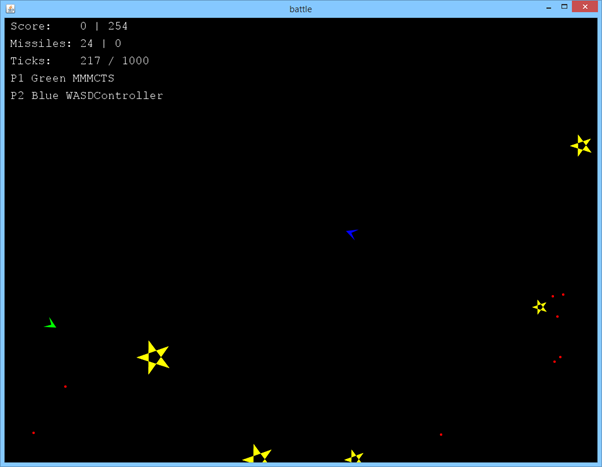
\includegraphics[scale=0.51]{resources/gamemode2}
		\caption{Without asteroids}
	\end{subfigure}
	\begin{subfigure}[b]{0.45\textwidth}
		\center
		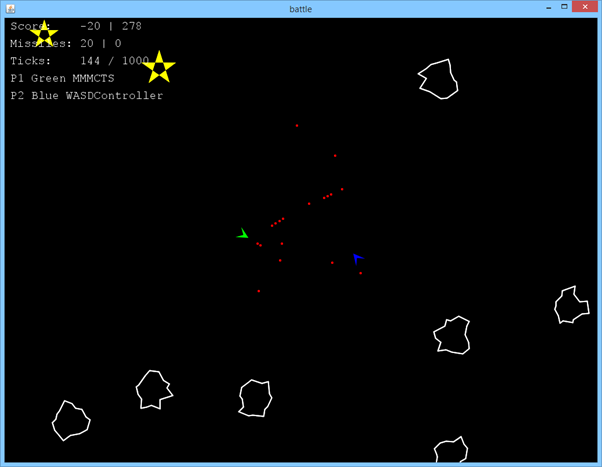
\includegraphics[scale=0.51]{resources/gamemode1}
		\caption{With simple\\asteroids}
	\end{subfigure}
	\begin{subfigure}[b]{0.45\textwidth}
		\center
		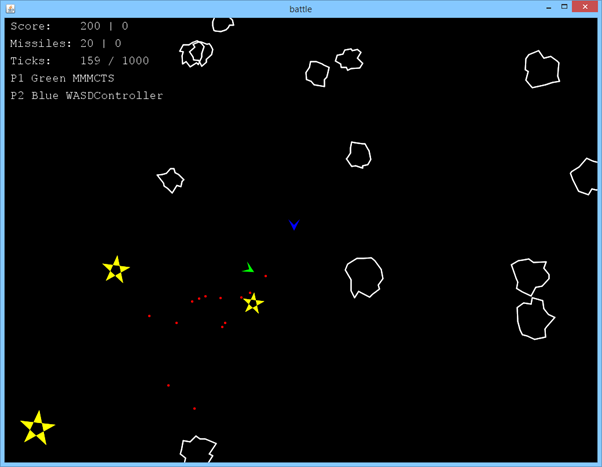
\includegraphics[scale=0.51]{resources/gamemode0}
		\caption{With splitting\\asteroids}
	\end{subfigure}
\end{figure}
	
%%%%%%%%%%%%%%%%%%%%%%%%%%%%%%%%%%%%%%%%%%%%%%%%%%%%%%%%%%%%%%%%%%%%%%%%%%%%%%%
\section{Analytics over AI agents}
\subsection{Motivation}
In order to try to confirm that the game variants generated had the intended effects on gameplay, we initially generated AI agents to play the games. We would then log the score, velocity, and missile count of each of the agents over the course of multiple runs, and use these results to try to try to quantify the effects of the variations in the game.

\subsection{Methodology}


For the purpose of testing the different variations of the game, 4 agents were used: MCTS with 40ms thinking time, MCTS with 20ms thinking time, RotateAndShoot and EmptyAI.
The assumption we made was that the 40ms MCTS would perform a lot better than the 20ms MCTS and that both would greatly overperform compared to RotateAndShoot and EmptyAI. The MCTS agents were also expected to perform admirably against human players.

During the IGGI Essex GD2 training courses, MCTS was found to be the best technique for this sort of game by far with 66 wins and only 4 losses in a round robin tournament between 7 algorithms. The next best AI managed 56 wins and 14 losses, but employed a lot of knowledge relevant to that simpler variation of Battle Asteroids. As a result of these findings, MCTS was picked as the only AI to challenge the game and the human players.

Both MCTS agents make use of a rollout depth of 16 and 3 macro actions. The use of macro actions allows the search space to grow more in a helpful manner, thus finding better moves overall. {Powley, E.J. and Whitehouse, D. and Cowling, P.I.} As mentioned previously, the only difference between them is the halved time to think the second agent has. This should, in theory, result in a worse performing agent, at least compared to the other agent.

RotateAndShoot employs a very simple behaviour: it is always rotating in one direction and it is always shooting. During the IGGI Essex GD2 trials, RotateAndShoot failed to beat any of the other AI implementations, but often did score positively regardless of eventual loss. Its inclusion helped demonstrate any clear differences in missile avoidance between the various game types and agents.

EmptyAI does nothing and is there to showcase the MCTS agents’ attempts at collecting as many points as possible, with minimal / no resistance from the opponent.

Following the IGGI Essex GD2 example, a round robin tournament was decided to test the 4 different agents competing against each other in all 3 variations of the game. This had two aims: to assess automated playability of each game variation, as well as understand how scoring affected changes between games. If the MCTS agents successfully collect a fair number of powerups and manage to hit the opponents often enough, while also avoiding asteroids (where applicable) and avoid being hit by the other player, one can assume the game is in a playable state. This must also be confirmed (or infirmed) by human testing.

The tournament consisted of each agent playing each other agent 30 times. This resulted in 180 matchups. Information about score over time, velocity over time and missiles left over time was stored (see figure X).

\subsection{Results}

Results of the tournament on the first variation of the game (asteroids that split) show the 40ms MCTS agent behaving best. This is as predicted, as the tree the algorithm can expand is much greater than the one the 20ms MCTS agent can create, thus being able to choose better moves every tick. 

This also proves the game will favour more skillful players to random ones and reward better play. The game is challenging enough that the weaker MCTS agent can still win, just not often enough compared to the one giving more thinking time.

\begin{figure}
	\caption{AI results over the game without}
	\begin{tabular}{p{7.5em} | p{4.5em} p{4.5em} p{4.5em} p{4.5em}}
		&
			Empty Controller &
			Rotate and Shoot &
			MCTS (20ns) &
			MCTS (40ms) \\ \hline
		Empty Controller &
			-&
			0\% &
			3\% &
			0\% \\
		Rotate and Shoot &
			1000\% &
			-&
			3\% &
			3\% \\ 
		MCTS (20ns) &
			97\% &
			97\% &
			-&
			30\% \\
		MCTS (40ns) &
			100\% &
			97\% &
			70\% &
			-\\
	\end{tabular}
\end{figure}

\begin{figure}
	\caption{AI results over the game with simple asteroids}
	\begin{tabular}{p{7.5em} | p{4.5em} p{4.5em} p{4.5em} p{4.5em}}
		&
			Empty Controller &
			Rotate and Shoot &
			MCTS (20ms) &
			MCTS (40ms) \\ \hline
		Empty Controller &
			-&
			0\% &
			0\% &
			0\% \\
		Rotate and Shoot &
			100\% &
			-&
			20\% &
			6\% \\ 
		MCTS (20ms) &
			100\% &
			80\% &
			-&
			57\% \\
		MCTS (40ms) &
			100\% &
			93\% &
			44\% &
			-\\
	\end{tabular}
\end{figure}

\begin{figure}
	\caption{AI results over the game with splitting asteroids}
	\begin{tabular}{p{7.5em} | p{4.5em} p{4.5em} p{4.5em} p{4.5em}}
		&
			Empty Controller &
			Rotate and Shoot &
			MCTS (20ms) &
			MCTS (40ms) \\ \hline
		Empty Controller &
			-&
			3\% &
			0\% &	
			0\% \\
		Rotate and Shoot &
			97\% &
			-&
			3\% &
			0\% \\ 
		MCTS (20ms) &
			100\% &
			97\% &
			-&
			30\% \\
		MCTS (40ms) &
			100\% &
			100\% &
			70\% &
			-\\
	\end{tabular}
\end{figure}

%%%%%%%%%%%%%%%%%%%%%%%%%%%%%%%%%%%%%%%%%%%%%%%%%%%%%%%%%%%%%%%%%%%%%%%%%%%%%%%
\section{Human playtesting}
\subsection{Human testing methodology}

32 participants recruited through opportunity sampling (21 male and 11 female, 29 Right Handed, 2 Left-Handed, 1 ambidextrous, ages ranging between 15 to 61, with Mean = 38.66 and SD = +-13.55). All participants provided written consent prior to the experiment and were properly debriefed about the purposes of the experiment afterwards. No deception was involved. A google document questionnaire was created to record the participants’ responses. No sensitive information was asked and the data recorded was fully anonymised. Participants played one version of our game and they subsequently filled out questions regarding that specific version before moving on the next one. For counterbalancing purposes we created 6 subconditions (ABC, ACB, BAC, BCA, CAB, CBA) in order to account for possible order-fatigue effects. These procedures were created to reflect best practices in research design. However, due to the limited time for experimentation and the small number of participants, which leads to low power, no meaningful inferences could be made.
%%%%%%%%%%%%%%%%%%%%%%%%%%%%%%%%%%%%%%%%%%%%%%%%%%%%%%%%%%%%%%%%%%%%%%%%%%%%%%%
\section{Future Work}
Lorem Ipsum

\subsection{Further work}

Lorem Ipsum

\printbibliography[heading=bibnumbered]

\end{document}